\documentclass[a4paper, 11pt, notitlepage, english]{article}

\usepackage{babel}
\usepackage[utf8]{inputenc}
\usepackage[T1]{fontenc, url}
\usepackage{textcomp}
\usepackage{amsmath, amssymb}
\usepackage{amsbsy, amsfonts}
\usepackage{graphicx, color}
\usepackage{parskip}
\usepackage{framed}
\usepackage{amsmath}
\usepackage{xcolor}
\usepackage{multicol}
\usepackage{url}
\usepackage{flafter}
\usepackage{caption}

%\DeclareCaptionLabelSeparator{colon}{. }
\renewcommand{\captionfont}{\sffamily}
\renewcommand{\captionlabelfont}{\bf\sffamily}
\setlength{\captionmargin}{20pt}

\usepackage{geometry}
\geometry{headheight=0.01mm}
\geometry{top=24mm, bottom=29mm, left=39mm, right=39mm}

\renewcommand{\arraystretch}{1.2}
\setlength{\tabcolsep}{10pt}
\makeatletter
\renewcommand*\env@matrix[1][*\c@MaxMatrixCols c]{%
  \hskip -\arraycolsep
  \let\@ifnextchar\new@ifnextchar
  \array{#1}}
%
% Parametere for inkludering av kode fra fil
%
\usepackage{listings}

\DeclareMathAlphabet{\mathbfit}{OML}{cmm}{b}{it}

\definecolor{javared}{rgb}{0.6,0,0} % for strings
\definecolor{javagreen}{rgb}{0.25,0.5,0.35} % comments
\definecolor{javapurple}{rgb}{0.5,0,0.35} % keywords
\definecolor{javadocblue}{rgb}{0.25,0.35,0.75} % javadoc

\lstset{language=python,
basicstyle=\ttfamily\scriptsize,
keywordstyle=\color{javapurple},%\bfseries,
stringstyle=\color{javared},
commentstyle=\color{javagreen},
morecomment=[s][\color{javadocblue}]{/**}{*/},
% numbers=left,
% numberstyle=\tiny\color{black},
stepnumber=2,
numbersep=10pt,
tabsize=4,
showspaces=false,
captionpos=b,
showstringspaces=false,
frame= single,
breaklines=true}
%
% Definering av egne kommandoer og miljøer
%
\newcommand{\dd}[1]{\ \text{d}#1}
\newcommand{\f}[2]{\frac{#1}{#2}} 
\newcommand{\beq}{\begin{equation}}
\newcommand{\eeq}{\end{equation}}
\newcommand{\bra}[1]{\langle #1|}
\newcommand{\ket}[1]{|#1 \rangle}
\newcommand{\braket}[2]{\langle #1 | #2 \rangle}
\newcommand{\braup}[1]{\langle #1 \left|\uparrow\rangle\right.}
\newcommand{\bradown}[1]{\langle #1 \left|\downarrow\rangle\right.}
\newcommand{\av}[1]{\left| #1 \right|}
\newcommand{\op}[1]{\hat{#1}}
\newcommand{\braopket}[3]{\langle #1 | {#2} | #3 \rangle}
\newcommand{\ketbra}[2]{\ket{#1}\bra{#2}}
\newcommand{\pp}[1]{\frac{\partial}{\partial #1}}
\newcommand{\ppn}[1]{\frac{\partial^2}{\partial #1^2}}
\newcommand{\up}{\left|\uparrow\rangle\right.}
\newcommand{\upup}{\left|\uparrow\uparrow\rangle\right.}
\newcommand{\down}{\left|\downarrow\rangle\right.}
\newcommand{\downdown}{\left|\downarrow\downarrow\rangle\right.}
\newcommand{\updown}{\left|\uparrow\downarrow\rangle\right.}
\newcommand{\downup}{\left|\downarrow\uparrow\rangle\right.}
\newcommand{\bupup}{\left.\langle\uparrow\uparrow\right|}
\newcommand{\bdowndown}{\left.\langle\downarrow\downarrow\right|}
\newcommand{\bupdown}{\left.\langle\uparrow\downarrow\right|}
\newcommand{\bdownup}{\left.\langle\downarrow\uparrow\right|}
\renewcommand{\d}{{\rm d}}
\newcommand{\Res}[2]{{\rm Res}(#1;#2)}
\newcommand{\To}{\quad\Rightarrow\quad}
\newcommand{\eps}{\epsilon}
\newcommand{\inner}[2]{\langle #1 , #2 \rangle}


\newcommand{\bt}[1]{\boldsymbol{#1}}
\newcommand{\mat}[1]{\textsf{\textbf{#1}}}
\newcommand{\I}{\boldsymbol{\mathcal{I}}}
\newcommand{\p}{\partial}
%
% Navn og tittel
%
\author{Jonas van den Brink \\ \texttt{j.v.d.brink@fys.uio.no}}
\title{Introduksjon til vitenskapelig programmering \\ Uke 2 \\ Sandvika vgs}

\begin{document}
\maketitle

Sist uke så vi på våre første kodesnutter og lærte å lage enkle programmer. Vi lærte hvordan vi skriver korte scripts ved å gi datamaskinen en rekke med kommandoer, og hvordan disse tolkes av maskinen når vi kjører programmet vårt. Vi så også på variable og typer, hvordan disse lages og brukes i programmering. Idag går vi videre med litt mer sammensatt programmering, vi kommer til å få bruk for alt vi har lært til nå, så vi kommer til å få god repetisjon av forrige ukes stoff på kjøpet. 

\clearpage

\section{Løkker}
Når vi ønsker å gjenta biter med kode, bruker vi gjerne noe som kalles en løkke, eller \emph{loop} på engelsk. I python har vi to typer løkken, og de er \emph{for}-løkken, og \emph{while}-løkken. I dag kommer vi bare til å se på for-løkker. En for løkke itererer over elementer i en liste, og utfører de samme kommandoene for hvert element.

La oss se på et enkelt eksempel
\begin{lstlisting}
for name in ['John', 'Mary', 'Lucy', 'Roger']:
    print name    
\end{lstlisting}
\vspace{-0.3cm}
Vi ser at vi starter en for-løkke med ordet \verb+for+, vi gir så navn til elementet, her har vi gitt det navnet \verb+name+, og så skriver vi kommandoen \verb+in+ og spesifiserer en liste. Nå kjøres all koden med innrykk om igjen for hvert element i lista. Resultatet av denne kodesnutten blir altså
\begin{lstlisting}
John
Mary
Lucy
Roger
\end{lstlisting}
\vspace{-0.3cm}
Merk at vi når vi definerte for-løkka skrev lista vi iterer over rett inn, vi skal selvfølgelig også lagre listen som en variabel, og gi variabelen, altså som følger:
\begin{lstlisting}
names = ['John', 'Mary', 'Lucy', 'Roger']

for name in names:
    print name    
\end{lstlisting}
\vspace{-0.3cm}


\subsection{Range}
Ofte når vi bruker løkker i programmeringssammenheng, er vi interessert i å iterere over en liste med tall. Det kan derfor være lurt å ha måter å lage store lister med tall på en enkel måte. For å gjøre dette kommer vi til å bruke Python-funksjonen \verb+range+. Vi må fortelle range hvor vi vil at listen skal begynne, hvor den skal slutte, og hvor store steg den skal ta. Ved default vil den begynne på 0 og ta steg på 1, så de tre kommandoene
\begin{lstlisting}
print range(10)     # gir stop = 10
print range(0,10)   # gir start = 0, stop = 10
print range(0,10,1) # gir start = 0, stop = 10, step = 1
\end{lstlisting}
\vspace{-0.3cm}
gir det samme resultatet, nemlig
\begin{lstlisting}
[0, 1, 2, 3, 4, 5, 6, 7, 8, 9]
\end{lstlisting}
\vspace{-0.3cm}
Merk at listen sluttet på 9, og ikke 10, \verb+range+-kommandoen gir altså en liste fra og med \verb+start+, til (men ikke med) \verb+stop+, med steg på \verb+step+. La oss se på et par flere eksempler:
\begin{lstlisting}
print range(1,10)
>>> [1, 2, 3, 4, 5, 6, 7, 8, 9]
\end{lstlisting}
\vspace{-0.3cm}
\begin{lstlisting}
print range(1,10,2)
>>> [1, 3, 5, 7, 9]
\end{lstlisting}
\vspace{-0.3cm}
\begin{lstlisting}
print range(-10,10,5)
>>> [-10, -5, 0, 5]
\end{lstlisting}
\vspace{-0.3cm}
\begin{lstlisting}
print range(10, 4, -1)
[10, 9, 8, 7, 6, 5]
\end{lstlisting}
\vspace{-0.3cm}
\begin{lstlisting}
print range(3,30,3)
[3, 6, 9, 12, 15, 18, 21, 24, 27]
\end{lstlisting}
\vspace{-0.3cm}
\begin{lstlisting}
print range(100)
[0, 1, 2, 3, 4, ..., 92, 93, 94, 95, 96, 97, 98, 99]
\end{lstlisting}
\vspace{-0.3cm}
Ved å bruke \verb+range+-kommandoen på riktig vis, kan vi altså lage lister med tall på en rask måte.


\subsection{Eksempel: Matematiske summer}
Som et eksempel, la oss bruke en løkke til å regne ut summen av tallene fra og med 1 til og med 1000. Det vil si:
$$S = \sum_{i=1}^{1000} i = 1 + 2 + 3 + \ldots + 998 + 999 + 1000.$$
I python, kan vi finne denne summen med følgende kodesnutt
\begin{lstlisting}
S = 0
for i in range(1,1001):
    S += i

print S
\end{lstlisting}
\vspace{-0.3cm}
som gir svaret
$$S = \sum_{i=1}^{1000} i = 500500.$$
Dette svaret kunne vi også ha funnet forholdsvis enkelt ved regne ut gjennomsnittet av alle tallene og gange med antall tall:
$$S = \frac{1+1000}{2}\cdot 1000 = 500500.$$
Flott! Svarene våres er enige. Som tyder på at koden vår gjorde akkurat det vi ville at den skulle gjøre. Nå kan vi regne ut et par summer ved hjelp av datamaskin som er langt vanskligere å regne ut for hånd.

La oss først se på den samme summen, men regne ut kvadratet av tallene, altså
$$S = \sum_{i=1}^{1000} i^2 = 1 + 4 + 9 + 16 + \ldots + 1000^2.$$
For å finne denne summen kan vi bruke nesten identisk kode som tidligere, vi må bare endre uttrykket inne i løkka
\begin{lstlisting}
S = 0
for i in range(1,1001):
    S += i**2

print S
\end{lstlisting}
\vspace{-0.3cm}
som gir svaret
$$S = \sum_{i=1}^{1000} i^2 = 333833500.$$
Denne summen var det altså like lett å finne numerisk, men for hånd er det langt vanskligere en den enklere summen.

\clearpage


\section{Funksjoner}
Du er kanskje vandt med navnet "funksjon" fra matematikk. Vi skal nå vise hvordan vi kan definere funksjoner i Python. Funksjoner i programmeringssammenheng er noe bredere enn matematiske funksjoner, men vi kommer fort til å se at de har mye til felles.

Den enkleste måten å tenke på en funksjon, er å se på det som en maskin, som tar noe input, for eksempel et tall, og så gir noe output, bestemt av inputten.
\begin{center}
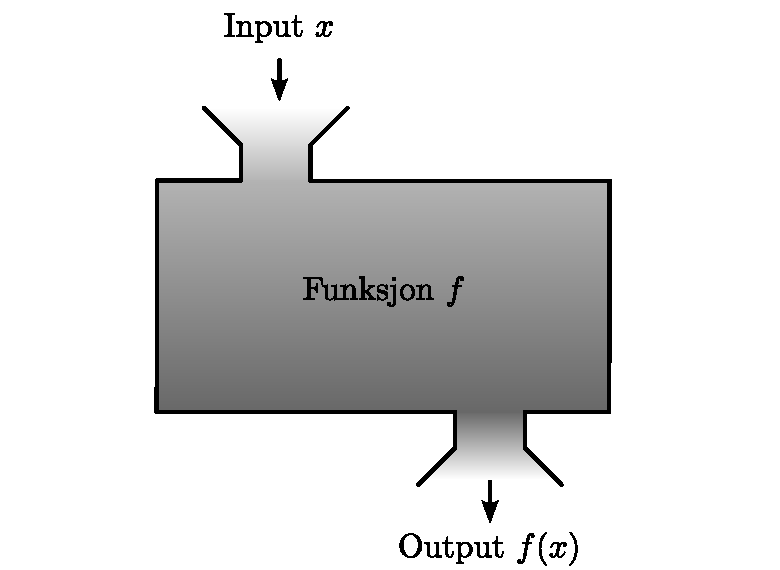
\includegraphics[width=0.8\textwidth]{function_blackbox}    
\end{center}

Hvis vi for eksempel ser på den matematiske funksjonen
$$f(x) = x^2 + 3x + 1.$$
Så kan vi for hver verdi av $x$ (input) beregne en resulterende verdi av $f(x)$ (output). Med andre ord er funksjonen $f$ en slags regel, eller maskin, som behandler et tall vi gir den. Vi kan definere denne funksjonen i Python som følger
\begin{lstlisting}
def f(x):
    return x**2 + 3*x + 1    
\end{lstlisting}
\vspace{-0.3cm}
her er \verb+def+ og \verb+return+ Python-kommandoer som vi skal forklare litt mer i detalj snart. Kort fortalt definerer vi her at det skal finnes en funksjon som heter $f$, som tar et tall $x$ inn, og gir tilbake (returnerer) tallet $f(x)$. Vi kan bruke funksjonen, vi kaller dette gjerne å "kalle på funksjonen", som følger
\begin{lstlisting}
print f(2)
print f(3.5)
print f(-1) + f(1)
\end{lstlisting}
\vspace{-0.3cm}
som gir:
\begin{lstlisting}
11
23.75
4
\end{lstlisting}
\vspace{-0.3cm}
Så fort vi har definert en funksjon i python, huskes denne helt til programmet er ferdig å kjøre, og vi kan bruke den så mye vi ønsker. Funksjoner vi definerer, er egentlig bare en ny type variabel.

En funksjon i python, trenger ikke nødvendigvis å være matematisk. Vi kan for-eksempel lage en funksjon som følger
\begin{lstlisting}
def greet(name):
    print "Hello " + name + "!"
\end{lstlisting}
\vspace{-0.3cm}
Denne funksjonen tar et navn som input, det vil si, en tekst-streng, og skriver ut en hilsen som output. Kommandoen
\begin{lstlisting}
greet("Lucy")
\end{lstlisting}
\vspace{-0.3cm}
resulterer altså i
\begin{lstlisting}
Hello Lucy!
\end{lstlisting}
\vspace{-0.3cm}
Merk at denne funksjonen ikke brukte kodenavnet \verb+return+, og når vi kallet på funksjonen, skrev vi ikke \verb+print+ før funksjonskallet. Dette er fordi funksjonen i seg selv printet, det var det vi hadde \emph{definert} at den skulle gjøre. Det er kanskje litt vanskelig å skjønne denne forskjellen, så la oss se på et par eksempler til.

Vi definerer to funksjoner, $f_1$ og $f_2$. Vi vil at de begge skal ta et tall $x$ som input, og regne ut $2x$, altså det dobbelte. Forskjellen skal være at $f_1$ returnerer resultatet, mens $f_2$ printer det. Vi har altså:
\begin{lstlisting}
def f1(x):
    return 2*x

def f2(x):
    print 2*x
\end{lstlisting}
\vspace{-0.3cm}
La oss nå prøve å kalle på $f_1$ og $f_2$ på forskjellige måter og prøve å forstå hva som skjer. Først skriver vi:
\begin{lstlisting}
f1(2)
\end{lstlisting}
\vspace{-0.3cm}
Vi får ikke noen feilmelding, så det virker greit. Men vi får heller ingen utskrift, det skjer ingenting! Dette er fordi vi kaller på $f_1$ med tallet 2 som input, funksjonen regner ut at $2*2 = 4$, og returnerer verdien, men så gjør vi ingenting med denne verdien. Vi kunne for eksempel gjort
\begin{lstlisting}
a = f1(2)
print a
\end{lstlisting}
\vspace{-0.3cm}
Her lagrer vi den returnerte verdien i en variabel \verb+a+, og så skriver vi ut \verb+a+. Nå får vi resultatet til skjerm, som er 4, flott!

La oss nå prøve
\begin{lstlisting}
f2(3)
\end{lstlisting}
\vspace{-0.3cm}
Dette fungerer veldig fint, vi får resultatet 6, rett til skjerm, flotte saker. Dette er fordi vi kaller på funksjonen $f_2$, som skriver tallet rett til skjermen. Om vi nå derimot prøver å lagre resultatet i en variabel
\begin{lstlisting}
a = f2(3)
print a
\end{lstlisting}
\vspace{-0.3cm}
får vi et litt mystisk resultat:
\begin{lstlisting}
6
None
\end{lstlisting}
\vspace{-0.3cm}
For å skjønne hva som skjer her, så må vi først tolke kodelinjen \verb+a = f2(3)+, som vi lærte forrige uke, så betyr en slik linje at vi skal regne ut det som er på høyre-siden, og lagre det i variabelen \verb+a+. Vel, på høyre side kaller vi på $f_2$ med tallet $x=3$, $f_2$ gjør som vi har definert å skriver ut resultatet $2*x=6$ rett til skjerm. Etter det er $f_2$ ferdig, men den har ikke \emph{returnert} noen verdi, så når \verb+a+ settes lik resultatet på høyre-siden, så blir den ingenting, eller \verb+None+ som det heter i Python.

Du har forhåpentligvis fått en viss idé om hva det nå betyr at en funksjon returnerer en verdi ved hjelp av \verb+return+-kommandoen. Ikke få panikk om du synes dette er ganske forvirrende, forståelse kommer med tid i programmering, så du skjønner det nok bedre etter du har fått prøvd deg litt frem!

\subsection{Funksjoner av flere variabler}
Når man først vet hvordan man lager funksjoner i python, er det superenkelt å lage funksjoner av flere variabler. Vi kan for eksempel lage følgende funksjon
$$f(x,y) = 2x^2 + xy + 3,$$
som følger
\begin{lstlisting}
def f(x,y):
    return 2*x**2 + x*y + 3

print f(3,4)
\end{lstlisting}
\vspace{-0.3cm}
Tilsvarende kan vi lage funksjoner som ikke tar noen argumenter. Disse er kanskje mer nyttig i en programmeringssammenheng enn i en matematisk sammenheng. Vi kan foreksempel lage en funksjon
\begin{lstlisting}
def greet():
    print "Hey there! I hope you have a great day!"
\end{lstlisting}
\vspace{-0.3cm}
Merk at for å kalle på en slik funksjon, må vi fortsatt bruke parantesene, slik at et kall på \verb+greet+ skrives
\begin{lstlisting}
greet()
\end{lstlisting}

En ting det er verdt å merke seg er at mange av kommandoene vi har brukt i Python hitil, er funksjoner som er definert på akkurat den måten vi har lagt frem nå. For eksempel er \verb+range+ en funksjon, som vi kaller på når vi bruker. Når vi skriver; \verb+range(1,10,2)+ så gjør vi et funksjonskall med 3 inputtall.

\clearpage

\section{Arrays}

Vi skal snart gå inn på plotting i Python, som vil si å lage figurer. Men da bør vi først nevne \verb+arrays+. Arrays er en spesiell type liste ment for matematikk. I motsetning til lister, som kan inneholde forskjellig type innhold, så kan arrays bare inneholde tall. Lister kan også gjøres større og mindre ved å legge til eller slette elementer, mens arrays \emph{alltid} har samme antall elementer. Om vi lager en array med tusen tall, så vil den arrayen alltid ha tusen tall, vi kan derimot endre hvilke tall den inneholder.

Dere skal nå få se de to vanligste måtene å lage arrays på. Først, et tomt array. Ettersom at et array alltid har likt antall plasser, må vi spesifisere størrelsen på arrayet. Vi bruker kommandoen \verb+zeros+:
\begin{lstlisting}
x = zeros(3)    
\end{lstlisting}
\vspace{-0.3cm}
Variabelen \verb+x+ er nå et array, med tre elementer. Der alle er satt til tallet 0. Dette virker kanskje litt rart å gjøre, men vi kan nå endre spesifikke elementer ved å indeksere på følgende måte
\begin{lstlisting}
x[0] = 10
x[1] = 4
x[2] = 3
\end{lstlisting}
\vspace{-0.3cm}
Firkantparantesene kalles "indeksering", og brukes for å få tilgang til enkelt elementer av et array eller en liste. Python starter å telle på 0, så \verb+x[0]+ er det første elementet, og \verb+x[1]+ det andre, osv.
Om vi nå skriver \verb+print x+ får vi nå resultatet
\begin{lstlisting}
[ 10.   4.   3.]
\end{lstlisting}
\vspace{-0.3cm}

Neste måte lage et array på, er med funksjonen \verb+linspace+, som står for \emph{linear spacing}. Den tar tre inputparamtere: start, stop, antall.Om vi for eksempel skriver
\begin{lstlisting}
x = linspace(0,10,11)
print x
\end{lstlisting}
\vspace{-0.3cm}
får vi 
\begin{lstlisting}
[ 0.   0.2  0.4  0.6  0.8  1. ]
\end{lstlisting}
\vspace{-0.3cm}
Altså er \verb+x+ et array med 6 elementer, hvor det første elementet er 0, det siste 1, og de resterende er jevnt fordelt. Vi kommer til å se at linspace er veldig praktisk når vi skal plotte.

\subsection{Vektoriserte funksjoner}
En stor fordel med arrays, er at de er laget for å drive med matematikk. Arrays oppfører seg foreksempel akkurat som vektorer. Det betyr at vi kan for eksempel bruke arrays til å regne prikkprodukt og kryssprodukt
\begin{lstlisting}
u = array([1,-4,3])
v = array([3,2,-1])
print dot(u,v)
print cross(u,v)
\end{lstlisting}
\vspace{-0.3cm}
\begin{lstlisting}
-8
[-2 10 14]
\end{lstlisting}
\vspace{-0.3cm}

En annen veldig nyttig funksjonalitet, er at vi kan kalle på funksjoner med arrays som input, om vi for eksempel har laget funksjonen som vi så på tidligere
\begin{lstlisting}
def f(x):
    return x**2 + 3*x + 1
\end{lstlisting}
\vspace{-0.3cm}
så kan vi kalle på denne med et array som følger
\begin{lstlisting}
a = array([0,1,2,3,4,5])
print f(a)
\end{lstlisting}
\vspace{-0.3cm}
\begin{lstlisting}
[ 1  5 11 19 29 41]
\end{lstlisting}
\vspace{-0.3cm}
Det som skjer når vi kaller på funkjsonen med et array, er at Python regner ut resultatet element for element og returnerer et array med resultatene tilbake.

\section{Plotting}
Vi skal nå se på plotting i Python, som vil si å lage enkle figurer og grafer. Vi kommer til å tegne inn grafen vår i et koordinatsystem som vi er vant med fra matematikk. For å plotte bruker vi funksjonen \verb+plot+ fra pakken Pylab, som tar som input to lister, eller arrays, av tall. Vi kan altså for eksempel skrive
\begin{lstlisting}
plot([0,0.5,1], [2,4,6], 'x')
show()
\end{lstlisting}
\vspace{-0.3cm}
Her tegnes altså punktene (0,2), (0.5,4) og (1,6) inn i koordinatsystemet.
Vi må bruke kommandoen \verb+show()+ for å vise figurer vi har laget. Vi har også lagt inn tekstrengen \verb+'x'+ i plotte-kommandoen, det er for at den skal tenge punktene vi gir som kryss. Hvis vi ikke ber den tegne kryss, tegner den rett og slett rette streker mellom punktene.

Om vi har definert en funksjon, for eksempel:
$$f(x) = x^2 + 3x + 1,$$
som vi har sett på tidligere. Kan vi nå gjøre som følger
\begin{lstlisting}
def f(x):
    return x**2 + 3*x + 1

x = linspace(-6,6,1000)
y = f(x)

plot(x,y)
show()
\end{lstlisting}
\vspace{-0.3cm}
Her lager vi altså et sett med tusen punkter, som vi så plotter. Vi får dermed en fin figur av funksjonen $f(x)$. 

Tilsvarende kan vi lage plot av velkjente matematiske funksjoner, for eksempel sinus og cosinus.
\begin{lstlisting}
x = linspace(0,2*pi,1000)
plot(x,sin(x))
plot(x,cos(x))
show()
\end{lstlisting}
\vspace{-0.3cm}
Merk at siden vi ga to plotte kommandoer før vi brukte show, så får vi to kurver i samme figur.

Etter vi har lagd kurven ved å bruke \verb+plot+-kommandoen, og før vi bruker \verb+show+, så kan vi pynte på figuren vår. Vi kan for eksempel legge til navn på akser med
\begin{lstlisting}
xlabel('x')
ylabel('y')
\end{lstlisting}
\vspace{-0.3cm}
Vi kan lage tittel på figuren med \verb+title+-funksjonen på samme måte. Vi kan definere hvilke deler av figuren vi skal vise med \verb+axis+, for eksmepel
\begin{lstlisting}
axis([0,2*pi,-1,1])
\end{lstlisting}
\vspace{-0.3cm}
vi gir altså en liste med \verb+[xstart, xstop, ystart, ystop]+.

Vi kan også lagre figuren vår med
\begin{lstlisting}
savefig('figure1.png')
savefig('figure1.pdf')
\end{lstlisting}
\vspace{-0.3cm}
som lagrer bilde som filene 'figure1.png' og 'figure2.pdf' henholdsvis.

Det er mange andre muligheter for å pynte på plot og få dem til å se kule ut, men la oss ikke dykke for dypt inn i det akkurat nå. Vi kommer til å se mer på plotte-muligheter iløpet av ukene som kommer, men om du er utålmodig kan du se på \url{matplotlib.org} som er nettsiden til plottepakken som pylab bruker, der finnes det mange eksempler på plots man kan lage.



\clearpage


\section*{Oppgave 1}
\begin{itemize}
\item[(a)] Definer en funksjon \verb+celsius_to_fahrenheit+ som tar grader $C$ som input, og returnerer grader Fahrenheit. Vi minner om at formelen for omregningen er
$$F = \frac{9}{5}C + 32.$$
\item[(b)] Bruk funksjonen til å finne ut hvor mange grader Fahrenheit disse tempraturene er: $20^\circ$, $0^\circ$, $-40^\circ$. 
\item[(c)] Skriv en løkke der du lar gradier i Celsius gå fra -100 til 100 og skriv ut de tilhørende gradene i Fahrenheit ved å bruke funksjonen din. \\ \textbf{Hint 1:} Bruk \texttt{range}-funksjonen \\
\textbf{Hint 2:} Du må kalle på funksjonen din inne i løkka.
\end{itemize}


\section*{Oppgave 2}
Vi skal nå bruke løkker og \verb+range+-funksjonen til å regne ut noen matematiske summer
\begin{itemize}
    \item[(a)] Regn ut summen av alle oddetall under 1000.
    \item[(b)] Regn ut summen av alle kvadrattall til og med 10000. \\ \textbf{Hint:} Vi er altså ute etter summen
    $$1 + 4 + 9 + 16 + \ldots + 10000 = \sum_{i=1}^{100} i^2.$$
    \item[(c)] Regn ut summen av den uendelige rekka
    $$1 + \frac{1}{2} + \frac{1}{4} + \frac{1}{8} + \ldots$$
    \textbf{Hint:} Hvert ledd i summen blir mindre og mindre, det holder altså å ta med for eksempel de 1000 første leddene. Da alle ledd etter dette vil bidra ekstremt lite til det endelige svaret
\end{itemize}

\section*{Oppgave 3}
\begin{itemize}
    \item[(a)] Plot $e^x$ for $x\in[0,2]$.
    \item[(b)] Lag et plot, der du viser de tre funksjonene:
    $$e^x, \qquad e^{-x}, \qquad 1/e^{x}.$$
    for $x \in [0,2]$. Her må du bruke \verb+axis+-kommandoen for å velge rimelige akser på figuren din!
    \item[(c)] Pynt på plottet du nettopp lagde ved hjelp av funksjonene \verb+axis+, \verb+xlabel+, \verb+legend+, \verb+title+ og \verb+grid+.
    \item[(d)] Lagre plottet ditt som en .pdf-fil, og som en .png-fil. Sjekk at filene ble lagret riktig og at de ser ut som forventet.
\end{itemize}



\clearpage

\section*{Utfordringer!}
\subsection*{Primtall}
Greier du å skrive en funksjon som tar et heltall som input, og finner ut om det er et primtall eller ikke?
\subsection*{Fibonacci}
Greier du å skrive et program som regner ut og skriver ut Fibonacci-tallene?
\subsection*{Project Euler}
På nettsiden \url{www.projecteuler.net} er det mange morsomme matematiske nøtter som er ment å løses ved programmering. Se om du greier å få til et par av de første oppgavene. Spør gjerne om hjelp.


\end{document}